\documentclass[spanish]{beamer}
\usepackage[spanish, activeacute]{babel}
\usepackage[latin1]{inputenc}
\usepackage{graphicx}

\usetheme{Ilmenau}

\title[Redes Neurales en Juegos]{Inteligencia Artificial II\\Redes Neurales en Juegos}
\author{Daniel Barreto \texttt{<daniel@ac.labf.usb.ve>}\\
        Kristoffer Pantic \texttt{<kristoffer.pantic@gmail.com>}}
\date{\today}

\begin{document}

\begin{frame}
\titlepage
\end{frame}

\begin{frame}[fragile]{Descripci�n General}
  \begin{itemize}
  \item Introducci�n
    \begin{itemize}
    \item Tipos de aprendizaje con redes neurales en juegos
    \end{itemize}

  \item Enfoques actuales
  
  \item Aplicaciones en estudio
    \begin{itemize}
    \item Aprendizaje en vivo (\emph{Online Learning})
    \item Aproximaciones centradas en el jugador
    \item Animaci�n inteligente de personajes
    \item Predicciones
    \item Estudios a nivel de inteligencia humana
    \end{itemize}
  \end{itemize}
\end{frame}

\begin{frame}{Introducci�n}
  \begin{figure}[htp]
    \centering
    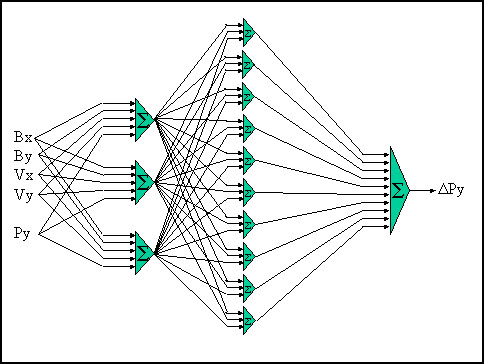
\includegraphics[scale=0.6]{media/neural.jpg}
  \end{figure}
\end{frame}

\begin{frame}{Tipos de aprendizaje en juegos}
  Particularmente para el aprendizaje artificial con redes neurales,
  podemos distinguir dos tipos aproximaciones:

  \begin{itemize}
  \item \emph{Offline learning.}
  \item \emph{Online learning.}
  \end{itemize}
\end{frame}

\begin{frame}{Tipos de aprendizaje en juegos}
  Otro tipo de categorizaci�n dada al aprendizaje artifical con redes
  neurales es:

  \begin{itemize}
  \item Aprendizaje supervisado
  \item Aprendizaje no supervisado
  \item Aprendizaje por reforzamiento
  \end{itemize}
\end{frame}

\begin{frame}{Enfoques actuales}
  
  \begin{itemize}
  \item Actualmente las redes neurales son poco usadas en juegos
    comerciales.
  \item En las versiones digitales de juegos de mesa como
    \emph{Othello}, \emph{Ajedrez}, \emph{Backgammon}, etc. es mas
    com�n el uso de redes neurales, por ser juegos de estrategia.
  \end{itemize}

  Los juegos de mesa suelen ser juegos m�s lentos con menos cambios de
  ambiente y mucha estrategia, mientras que en los juegos modernos hay
  muchos otros factores con que lidear aparte de la inteligencia
  artificial.
\end{frame}

\begin{frame}{Enfoques actuales}
  A pesar del poco uso, las redes neurales actualmente estan siendo
  utilizadas en el proceso de toma de decisiones de los agentes.
  \begin{figure}[htp]
    \centering
    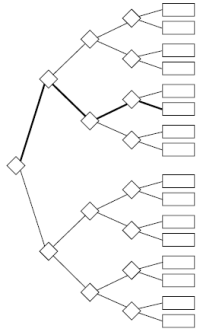
\includegraphics[scale=0.3,angle=270]{media/decision-tree.png}
  \end{figure}

  Los agentes procesan lo recibido por sus sensores, y a trav�s de una
  red entrenada (usualmente de forma \emph{offline}) toman acciones a
  partir de su output.\\

  Esto supone ahorro de c�digo y complejidad de maquinas de estados y
  agentes basados en reglas.
\end{frame}

\begin{frame}{Ejemplos de enfoques actuales}
  \begin{center}
    \textbf{Colin McRae Rally 2}
  \end{center}
  \begin{figure}[htp]
    \centering
    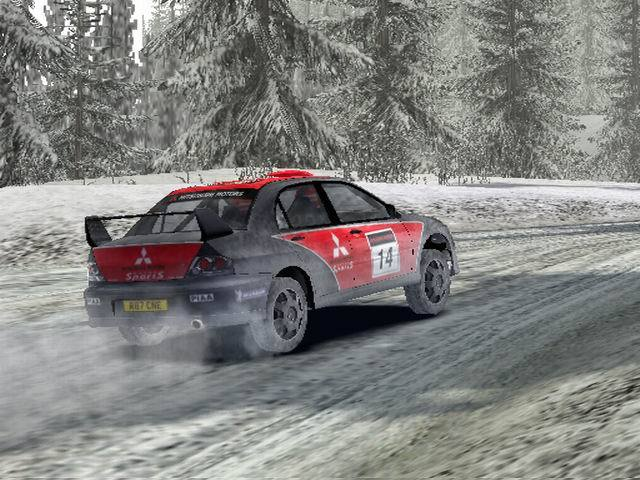
\includegraphics[scale=0.3]{media/colin-mcrae-rally.jpg}
  \end{figure}
\end{frame}

\begin{frame}{Ejemplos de enfoques actuales}
  \begin{center}
    \textbf{The Sims}
  \end{center}
  \begin{figure}[htp]
    \centering
    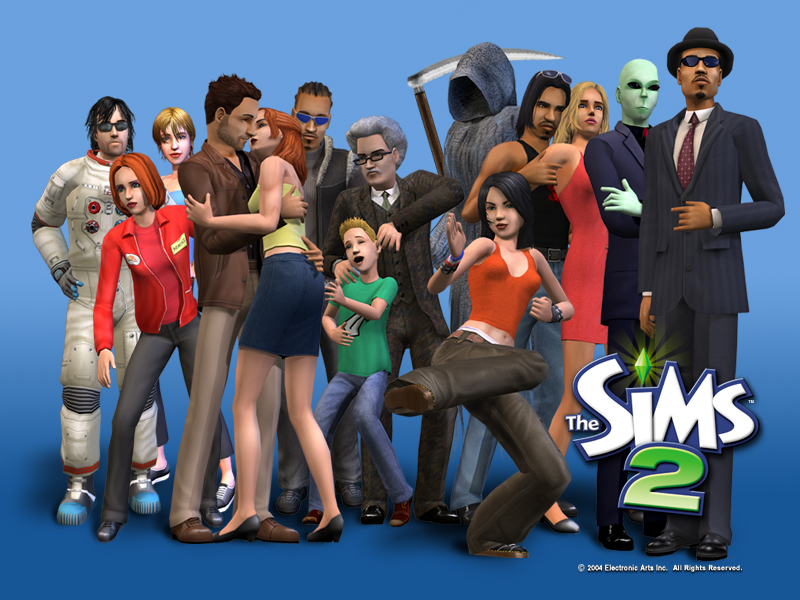
\includegraphics[scale=0.25]{media/the-sims.jpg}
  \end{figure}
\end{frame}

\begin{frame}{Ejemplos de enfoques actuales}
  \begin{center}
    \textbf{Creatures}
  \end{center}
  \begin{figure}[htp]
    \centering
    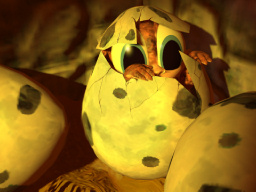
\includegraphics[scale=3.2]{media/creatures.jpg}
  \end{figure}
\end{frame}

\begin{frame}{Aplicaciones en estudio} 
  \begin{itemize}
  \item Aprendizaje en vivo (\emph{Online Learning})
  \item Aproximaciones centradas en el jugador
  \item Animaci�n inteligente de personajes
  \item Predicciones
  \item Estudios a nivel de inteligencia humana
  \end{itemize}
\end{frame}

\begin{frame}{Aprendizaje en vivo (\emph{Online Learning})}
  
\end{frame}

\begin{frame}{Aproximaciones centradas en el jugador}
  
\end{frame}

\begin{frame}{Animaci�n inteligente de personajes}
  
\end{frame}

\begin{frame}{Predicciones}
  
\end{frame}

\begin{frame}{Estudios a nivel de inteligencia humana}
  
\end{frame}

\end{document}